\chapter{Системный вызов open()} 

\noindent\textbf{Версия ядра:} \texttt{6.3.5}.

%везде написать на блоках "возврат чего-то там" конкретный тип возвращаемого значения

Системный вызов \texttt{open()} открывает файл, определённый \texttt{pathname}. Если указанный файл не существует и в \texttt{flags} указан флаг \texttt{O\_CREAT}, то \texttt{open()} может (необязательно) создать указанный файл с правами доступа, определёнными \texttt{mode}. Если флаг \texttt{O\_CREAT} не указан, параметр \texttt{mode} игнорируется.

\begin{lstlisting}
	int open(const char *pathname, int flags, mode_t mode);
\end{lstlisting}

\section{Возвращаемое значение}

\texttt{open()} возвращает файловый дескриптор~---~небольшое неотрицательное целое число, которое является ссылкой на запись в системной таблице открытых файлов и индексом записи в таблице дескрипторов открытых файлов процесса. Этот дескриптор используется далее в системных вызовах \texttt{read()}, \texttt{write()}, \texttt{lseek()}, \texttt{fcntl()} и т.д. для ссылки на открытый файл. В случае успешного вызова будет возвращён наименьший файловый дескриптор, не связанный с открытым процессом файлом.

В случае ошибки возвращается \texttt{-1} и устанавливается значение \texttt{errno}.

\section{Параметры}

\texttt{pathname}~---~имя файла в файловой системе. \texttt{flags}~---~режим открытия файла~---~один или несколько флагов открытия, объединенных оператором \textbf{побитового или}. 

\section{Флаги}

\begin{itemize}
	\item \texttt{O\_RDONLY}~---~открыть только для чтения.
	\item \texttt{O\_WRONLY}~---~открыть только для записи.
	\item \texttt{O\_RDWR}~---~открыть для чтения и записи.
	\item \texttt{O\_EXEC}~---~открыть только для выполнения (результат не определен при открытии директории).
	\item \texttt{O\_SEARCH}~---~открыть директорию только для поиска (результат не определен при использовании с файлами, не являющимися директорией).
	\item \texttt{O\_APPEND}~---~открыть в режиме добавления, перед каждой операцией записи файловый указатель будет устанавливаться в конец файла.
	\item \texttt{O\_CLOEXEC}~---~устанавливает флаг \texttt{close-on-exec} для нового файлового дескриптора (при вызове \texttt{exec} файл не будет оставаться открытым).
	\item \texttt{O\_CREAT}~---~если файл не существует, то он будет создан с правами доступа, определёнными \texttt{mode}.
	\item \texttt{O\_DIRECTORY}~---~вернуть ошибку, если файл не является каталогом.
	\item \texttt{O\_DSYNC}~---~файл открывается в режиме синхронного ввода-вывода (все операции записи для соответствующего дескриптора файла блокируют вызывающий процесс до тех пор, пока данные не будут физически записаны).
	\item \texttt{O\_EXCL}~---~при использовании совместно с \texttt{O\_CREAT} вернуть ошибку, если файл уже существует.
	\item \texttt{O\_NOATIME}~---~не обновлять время последнего доступа к файлу.
	\item \texttt{O\_NOCTTY}~---~если файл указывает на терминальное устройство, то оно не станет терминалом управления процесса, даже при его отсутствии.
	\item \texttt{O\_NOFOLLOW}~---~вернуть ошибку, если часть пути является символической ссылкой.
	\item \texttt{O\_NONBLOCK}~---~файл открывается, по возможности, в режиме \texttt{non-blocking}, то есть никакие последующие операции над дескриптором файла не заставляют вызывающий процесс ждать.
	\item \texttt{O\_RSYNC}~---~операции записи должны выполняться на том же уровне, что и \texttt{O\_SYNC}.
	\item \texttt{O\_SYNC}~---~файл открывается в режиме синхронного ввода-вывода (все операции записи для соответствующего дескриптора файла блокируют вызывающий процесс до тех пор, пока данные не будут физически записаны).
	\item \texttt{O\_TRUNC}~---~если файл уже существует, он является обычным файлом и заданный режим позволяет записывать в этот файл, то его длина будет урезана до нуля.
	\item \texttt{O\_LARGEFILE}~---~позволяет открывать файлы, размер которых не может быть представлен типом \texttt{off\_t (long)}. Для установки должен быть указан макрос \\ \texttt{\_LARGEFILE64\_SOURCE}.
	\item \texttt{O\_TMPFILE}~---~создать неименованный временный файл;
	\item \texttt{O\_PATH}~---~получить файловый дескриптор, который можно использовать для двух целей: для указания положения в дереве файловой системы и для выполнения операций, работающих исключительно на уровне файловых дескрипторов. Если \texttt{O\_PATH} указан, то биты флагов, отличные от \texttt{O\_CLOEXEC}, \texttt{O\_DIRECTORY} и \texttt{O\_NOFOLLOW}, игнорируются.
\end{itemize}

Если указан флаг \texttt{O\_CREAT}, вызов \texttt{open()} создает новый файл с правами из  \texttt{mode}:

\begin{itemize}
	\item \texttt{S\_IRWXU}~---~права на чтение, запись, выполнение для пользователя.
	\item \texttt{S\_IRUSR}~---~права на чтение для пользователя.
	\item \texttt{S\_IWUSR}~---~права на запись для пользователя.
	\item \texttt{S\_IXUSR}~---~права на выполнение для пользователя.
	\item \texttt{S\_IRWXG}~---~права на чтение, запись, выполнение для группы.
	\item \texttt{S\_IRGRP}~---~права на чтение для группы.
	\item \texttt{S\_IWGRP}~---~права на запись для группы.
	\item \texttt{S\_IXGRP}~---~права на выполнение для группы.
	\item \texttt{S\_IRWXO}~---~права на чтение, запись, выполнение для остальных.
	\item \texttt{S\_IROTH}~---~права на чтение для остальных.
	\item \texttt{S\_IWOTH}~---~права на запись для остальных.
	\item \texttt{S\_IXOTH}~---~права на выполнение для остальных.
	\item \texttt{S\_ISUID}~---~бит \texttt{set-user-ID}.
	\item \texttt{S\_ISGID}~---~бит \texttt{set-group-ID}.
	\item \texttt{S\_ISVTX}~---~«липкий» бит.
\end{itemize}

\chapter{Структуры}

\section{open\_how}

\begin{lstlisting}
	struct open_how {
	__u64 flags;
	__u64 mode;
	__u64 resolve; 
};
\end{lstlisting}

\section{open\_flags}

\begin{lstlisting}
struct open_flags {
	int open_flag;
	umode_t mode;
	int acc_mode;
	int intent;
	int lookup_flags;
};
\end{lstlisting}

\section{VALID\_OPEN\_FLAGS}

\begin{lstlisting}
#define S_IRWXUGO	(S_IRWXU|S_IRWXG|S_IRWXO)
#define S_IALLUGO	(S_ISUID|S_ISGID|S_ISVTX|S_IRWXUGO)

#define VALID_OPEN_FLAGS (O_RDONLY | O_WRONLY | O_RDWR | O_CREAT | O_EXCL | O_NOCTTY | O_TRUNC | O_APPEND | O_NDELAY | O_NONBLOCK | __O_SYNC | O_DSYNC | FASYNC	| O_DIRECT | O_LARGEFILE | O_DIRECTORY | O_NOFOLLOW | O_NOATIME | O_CLOEXEC | O_PATH | __O_TMPFILE)
\end{lstlisting}

\section{filename}

\begin{lstlisting}
struct filename {
	const char		*name;	/* pointer to actual string */
	const __user char	*uptr;	/* original userland pointer */
	int			refcnt;
	struct audit_names	*aname;
	const char		iname[];
};
\end{lstlisting}

\section{file}

\begin{lstlisting}
struct file {
	union {
		struct llist_node	f_llist;
		struct rcu_head 	f_rcuhead;
		unsigned int 		f_iocb_flags;
	};
	struct path		f_path;
	struct inode		*f_inode;	/* cached value */
	const struct file_operations	*f_op;
	/*
	 * Protects f_ep, f_flags.
	 * Must not be taken from IRQ context.
	 */
	spinlock_t		f_lock;
	atomic_long_t		f_count;
	unsigned int 		f_flags;
	fmode_t			f_mode;
	struct mutex		f_pos_lock;
	loff_t			f_pos;
	struct fown_struct	f_owner;
	const struct cred	*f_cred;
	struct file_ra_state	f_ra;
	u64			f_version;
#ifdef CONFIG_SECURITY
	void			*f_security;
#endif
	/* needed for tty driver, and maybe others */
	void			*private_data;
#ifdef CONFIG_EPOLL
	/* Used by fs/eventpoll.c to link all the hooks to this file */
	struct hlist_head	*f_ep;
#endif /* #ifdef CONFIG_EPOLL */
	struct address_space	*f_mapping;
	errseq_t		f_wb_err;
	errseq_t		f_sb_err; /* for syncfs */
} __randomize_layout
  __attribute__((aligned(4)));	/* lest something weird decides that 2 is OK */
\end{lstlisting}

\section{files\_struct}

\begin{lstlisting}
	/*
 * Open file table structure
 */
struct files_struct {
  /*
   * read mostly part
   */
	atomic_t count;
	bool resize_in_progress;
	wait_queue_head_t resize_wait;

	struct fdtable __rcu *fdt;
	struct fdtable fdtab;
  /*
   * written part on a separate cache line in SMP
   */
	spinlock_t file_lock ____cacheline_aligned_in_smp;
	unsigned int next_fd;
	unsigned long close_on_exec_init[1];
	unsigned long open_fds_init[1];
	unsigned long full_fds_bits_init[1];
	struct file __rcu * fd_array[NR_OPEN_DEFAULT];
};
\end{lstlisting}

\section{fdtable}

\begin{lstlisting}
struct fdtable {
	unsigned int max_fds;
	struct file __rcu **fd;      /* current fd array */
	unsigned long *close_on_exec;
	unsigned long *open_fds;
	unsigned long *full_fds_bits;
	struct rcu_head rcu;
};
\end{lstlisting}

\section{nameidata}

\begin{lstlisting}
#define EMBEDDED_LEVELS 2
struct nameidata {
	struct path	path;
	struct qstr	last;
	struct path	root;
	struct inode	*inode; /* path.dentry.d_inode */
	unsigned int	flags, state;
	unsigned	seq, next_seq, m_seq, r_seq;
	int		last_type;
	unsigned	depth;
	int		total_link_count;
	struct saved {
		struct path link;
		struct delayed_call done;
		const char *name;
		unsigned seq;
	} *stack, internal[EMBEDDED_LEVELS];
	struct filename	*name;
	struct nameidata *saved;
	unsigned	root_seq;
	int		dfd;
	vfsuid_t	dir_vfsuid;
	umode_t		dir_mode;
} __randomize_layout;

\end{lstlisting}

\section{LOOKUP\_REVAL и LOOKUP\_RCU}

\begin{lstlisting}
#define LOOKUP_REVAL		0x0020	/* tell ->d_revalidate() to trust no cache */
#define LOOKUP_RCU		0x0040	/* RCU pathwalk mode; semi-internal */
\end{lstlisting}

\texttt{LOOKUP\_RCU}~---~флаг используется в системе VFS для указания, что операция поиска должна выполняться с использованием RCU (\texttt{Read-Copy-Update}).
 
\texttt{LOOKUP\_REVAL}~---~флаг для работы с NFS, указывает не использовать кеш.

\texttt{O\_APPEND} может привести к потере данных в файловых системах NFS, если несколько процессов одновременно добавляют данные в файл. Это связано с тем, что NFS не поддерживает добавление данных в конец файла. Поэтому клиентское ядро должно имитировать этот флаг, что невозможно сделать без условия гонки. Клиент должен обеспечить монопольный доступ к файлу.

\section{dentry}

\begin{lstlisting}
struct dentry {
	/* RCU lookup touched fields */
	unsigned int d_flags;		/* protected by d_lock */
	seqcount_spinlock_t d_seq;	/* per dentry seqlock */
	struct hlist_bl_node d_hash;	/* lookup hash list */
	struct dentry *d_parent;	/* parent directory */
	struct qstr d_name;
	struct inode *d_inode;		/* Where the name belongs to - NULL is
					 * negative */
	unsigned char d_iname[DNAME_INLINE_LEN];	/* small names */

	/* Ref lookup also touches following */
	struct lockref d_lockref;	/* per-dentry lock and refcount */
	const struct dentry_operations *d_op;
	struct super_block *d_sb;	/* The root of the dentry tree */
	unsigned long d_time;		/* used by d_revalidate */
	void *d_fsdata;			/* fs-specific data */

	union {
		struct list_head d_lru;		/* LRU list */
		wait_queue_head_t *d_wait;	/* in-lookup ones only */
	};
	struct list_head d_child;	/* child of parent list */
	struct list_head d_subdirs;	/* our children */
	/*
	 * d_alias and d_rcu can share memory
	 */
	union {
		struct hlist_node d_alias;	/* inode alias list */
		struct hlist_bl_node d_in_lookup_hash;	/* only for in-lookup ones */
	 	struct rcu_head d_rcu;
	} d_u;
} __randomize_layout;
\end{lstlisting}



\chapter{Схема выполнения open()}

\section{open()}

\begin{table}[h!]
  \centering
  \begin{tabular}{p{1\linewidth}}
    \centering
    \includegraphics[width=0.8\linewidth]{./images/open.pdf}
    \captionof{figure}{open()}
    \label{img:er}
  \end{tabular}
\end{table} 

\newpage

\section{do\_sys\_open()}

\begin{table}[h!]
  \centering
  \begin{tabular}{p{1\linewidth}}
    \centering
    \includegraphics[width=0.7\linewidth]{./images/do\_sys\_open.pdf}
    \captionof{figure}{do\_sys\_open()}
    \label{img:er}
  \end{tabular}
\end{table}

\newpage

\section{build\_open\_how()}

\begin{table}[h!]
  \centering
  \begin{tabular}{p{1\linewidth}}
    \centering
    \includegraphics[width=0.8\linewidth]{./images/build\_open\_how.pdf}
    \captionof{figure}{build\_open\_how()}
    \label{img:er}
  \end{tabular}
\end{table}

\newpage

\section{do\_sys\_openat2()}

\begin{table}[h!]
  \centering
  \begin{tabular}{p{1\linewidth}}
    \centering
    \includegraphics[width=0.65\linewidth]{./images/do\_sys\_openat2.pdf}
    \captionof{figure}{do\_sys\_openat2()}
    \label{img:er}
  \end{tabular}
\end{table}

\newpage

\section{build\_open\_flags()}

\begin{table}[h!]
  \centering
  \begin{tabular}{p{1\linewidth}}
    \centering
    \includegraphics[width=1\linewidth]{./images/build\_open\_flags.pdf}
    \captionof{figure}{build\_open\_flags()}
    \label{img:er}
  \end{tabular}
\end{table}

\newpage

\begin{table}[h!]
  \centering
  \begin{tabular}{p{1\linewidth}}
    \centering
    \includegraphics[width=1\linewidth]{./images/build\_open\_flags2.pdf}
    \captionof{figure}{build\_open\_flags()}
    \label{img:er}
  \end{tabular}
\end{table}

\newpage

\section{getname\_flags()}

\begin{table}[h!]
  \centering
  \begin{tabular}{p{1\linewidth}}
    \centering
    \includegraphics[width=0.7\linewidth]{./images/getname\_flags.pdf}
    \captionof{figure}{getname\_flags()}
    \label{img:er}
  \end{tabular}
\end{table}

\newpage

\section{\_\_alloc\_fd()}

% тут поменять цикл на то, что она нарисовала

\begin{table}[h!]
  \centering
  \begin{tabular}{p{1\linewidth}}
    \centering
    \includegraphics[width=0.7\linewidth]{./images/alloc\_fd.pdf}
    \captionof{figure}{\_\_alloc\_fd()}
    \label{img:er}
  \end{tabular}
\end{table}

\newpage

\section{do\_filp\_open()}

\begin{table}[h!]
  \centering
  \begin{tabular}{p{1\linewidth}}
    \centering
    \includegraphics[width=0.7\linewidth]{./images/do\_filp\_open.pdf}
    \captionof{figure}{do\_filp\_open()}
    \label{img:er}
  \end{tabular}
\end{table}

\newpage

\section{\_\_set\_nameidata()}

\begin{table}[h!]
  \centering
  \begin{tabular}{p{1\linewidth}}
    \centering
    \includegraphics[width=0.7\linewidth]{./images/nameidata.pdf}
    \captionof{figure}{set\_nameidata()}
    \label{img:er}
  \end{tabular}
\end{table}

\newpage

\section{restore\_nameidata()}

\begin{table}[h!]
  \centering
  \begin{tabular}{p{1\linewidth}}
    \centering
    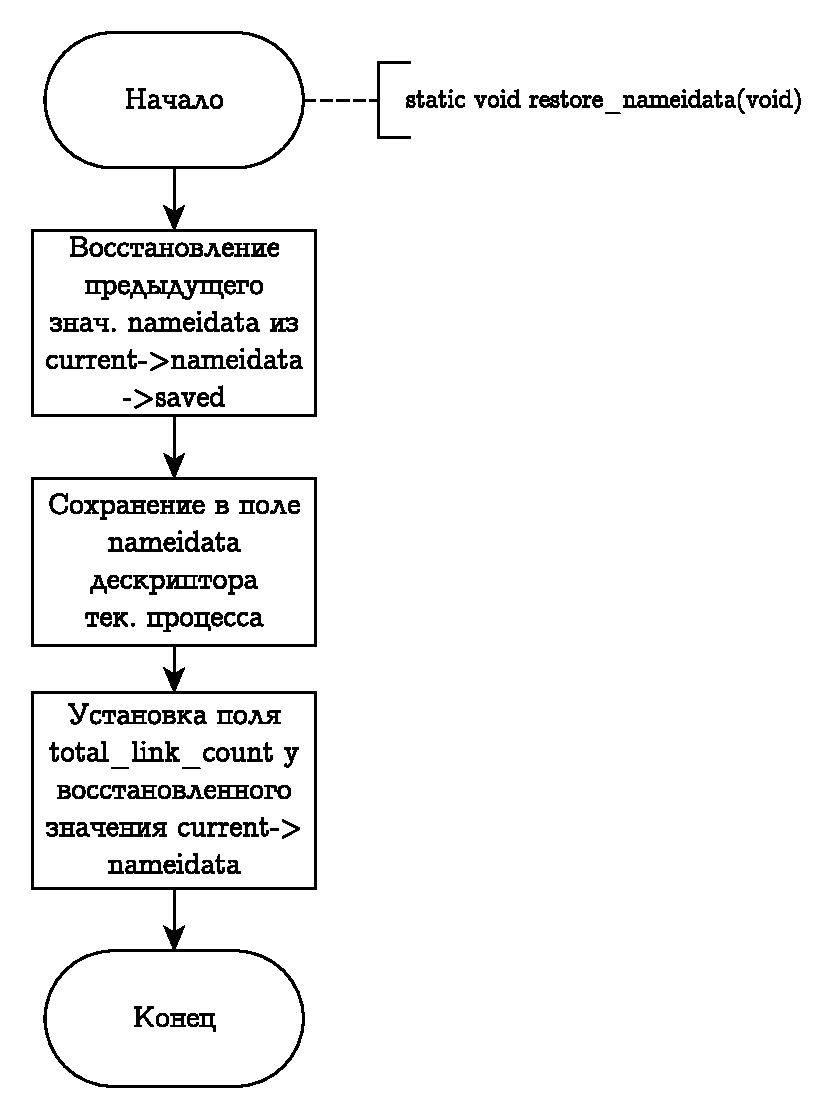
\includegraphics[width=0.7\linewidth]{./images/nameidata1.pdf}
    \captionof{figure}{restore\_nameidata()}
    \label{img:er}
  \end{tabular}
\end{table}

\newpage

\section{path\_openat()}

\begin{table}[h!]
  \centering
  \begin{tabular}{p{1\linewidth}}
    \centering
    \includegraphics[width=0.9\linewidth]{./images/path\_openat.pdf}
    \captionof{figure}{path\_openat()}
    \label{img:er}
  \end{tabular}
\end{table}

\newpage

\section{open\_last\_lookups()}

\begin{table}[h!]
  \centering
  \begin{tabular}{p{1\linewidth}}
    \centering
    \includegraphics[width=0.7\linewidth]{./images/open\_last\_lookups.pdf}
    \captionof{figure}{open\_last\_lookups()}
    \label{img:er}
  \end{tabular}
\end{table}

\newpage

\section{lookup\_open()}

% тут создание айнод поподробнее расписать

\begin{table}[h!]
  \centering
  \begin{tabular}{p{1\linewidth}}
    \centering
    \includegraphics[width=0.5\linewidth]{./images/lookup\_open.pdf}
    \captionof{figure}{lookup\_open()}
    \label{img:er}
  \end{tabular}
\end{table}

\newpage

\section{do\_open()}

\begin{table}[h!]
  \centering
  \begin{tabular}{p{1\linewidth}}
    \centering
    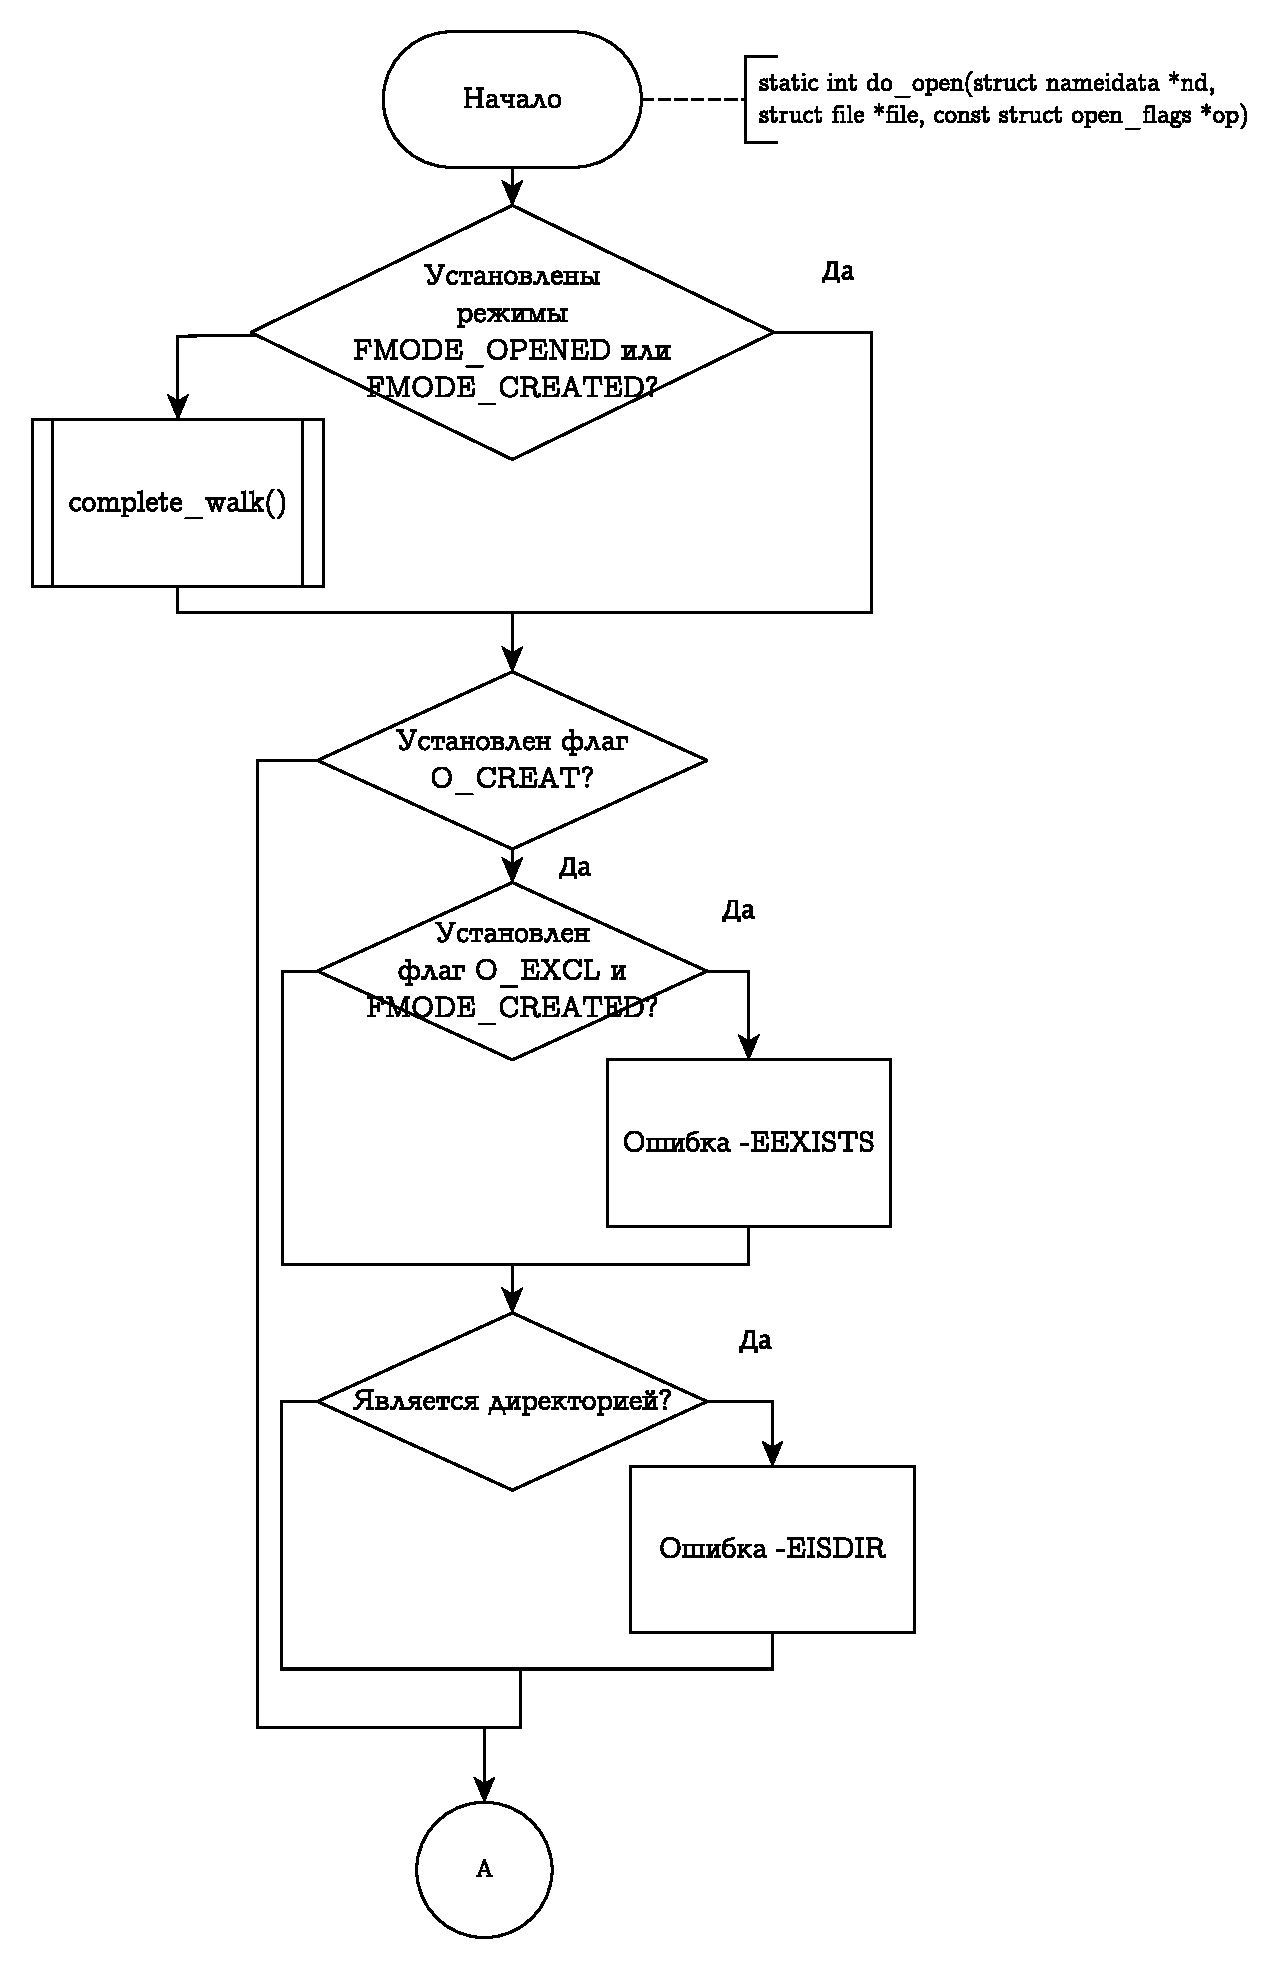
\includegraphics[width=0.7\linewidth]{./images/do_open.pdf}
    \captionof{figure}{do\_open()}
    \label{img:er}
  \end{tabular}
\end{table}

\newpage

\begin{table}[h!]
  \centering
  \begin{tabular}{p{1\linewidth}}
    \centering
    \includegraphics[width=0.55\linewidth]{./images/do\_open2.pdf}
    \captionof{figure}{do\_open()}
    \label{img:er}
  \end{tabular}
\end{table}

\newpage

\section{may\_open()}

\begin{table}[h!]
  \centering
  \begin{tabular}{p{1\linewidth}}
    \centering
    \includegraphics[width=0.8\linewidth]{./images/may\_open.pdf}
    \captionof{figure}{may\_open()}
    \label{img:er}
  \end{tabular}
\end{table}






